% DO NOT COMPILE THIS FILE DIRECTLY!
% This is included by the other .tex files.

\begin{frame}[t,plain]
\titlepage
\end{frame}

\begin{frame}
\frametitle{Objectives}
\begin{itemize}
        \item Learning how to use MISP to support common OSINT gathering use-cases as often used by SOC, CSIRTs and CERTs
        \item By using a list of practical exercise\footnote{\url{https://gist.github.com/adulau/8c1de48060e259799d3397b83b0eec4f}}
        \item The exercises are {\bf practical recent cases to model and structure intelligence} using the MISP standard
        \item Improving the data models available in MISP by exchanging live improvements and ideas
        \item Being able to share the results to the community at the end of this session
\end{itemize}
\end{frame}

\begin{frame}
\frametitle{(Threat) Intelligence}
\begin{itemize}
        \item {\bf Cyber threat intelligence (CTI) is a vast concept} which includes different fields such as intelligence as defined in the military community or in the financial sector or the intelligence community
        \item {\bf MISP project doesn't want to lock an organisation or an user into a specific model}. Each model is useful depending of the objectives from an organisation
        \item A set of pre-defined knowledge base or data-models are available and organisation can select (or create) what they need
        \item During this session, an overview of the most used taxonomies, galaxies and objects will be described
\end{itemize}
\end{frame}

\begin{frame}
\frametitle{Meta information and Contextualisation}
\begin{itemize}
\item Quality of indicators/attributes are important but {\bf tagging and classification are also critical to ensure actionable information}
        \item Tagging intelligence is done by using tags in MISP which are often originating from MISP taxonomy libraries
\end{itemize}
\end{frame}

\begin{frame}
\frametitle{microblog object}
\begin{columns}[totalwidth=\textwidth]
        \column{0.49\textwidth}\underline{Use case}\\
A serie of OSINT tweets from a security researcher.
To structure the thread, the information
and keep an history.\\
        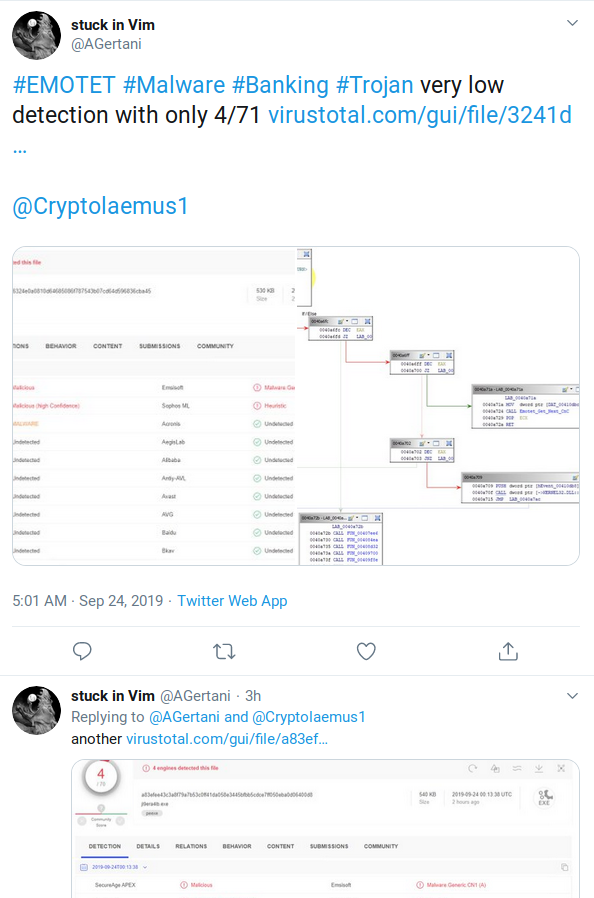
\includegraphics[scale=0.15]{emotet.png}
        \column{0.49\textwidth}\underline{Object to use}\\
        The microblog object can be used for Tweet or any microblog post (e.g. Facebook). Then object can be linked using {\it followed-by} to describe a serie of post.\\
        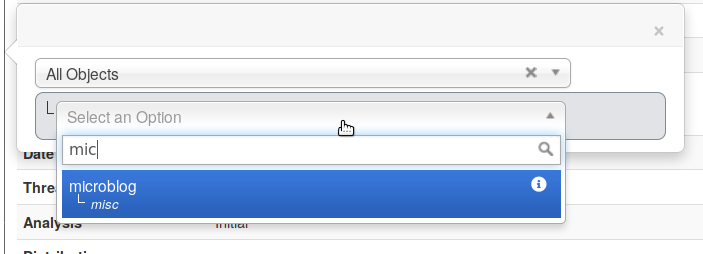
\includegraphics[scale=0.15]{microblog.png}
\end{columns}
\end{frame}


\begin{frame}
\frametitle{file object}
\begin{columns}[totalwidth=\textwidth]
        \column{0.49\textwidth}\underline{Use case}\\
        \begin{itemize}
                \item A file sample was received by email or extracted from VirusTotal.
                \item A list of file hashes were included in a report.
                \item A hash value was mentioned in a blog post.
        \end{itemize}
        \column{0.49\textwidth}\underline{Object to use}\\
        The file object can be used to describe file. It's usual to have partial meta information such as a single hash and a filename.\\
        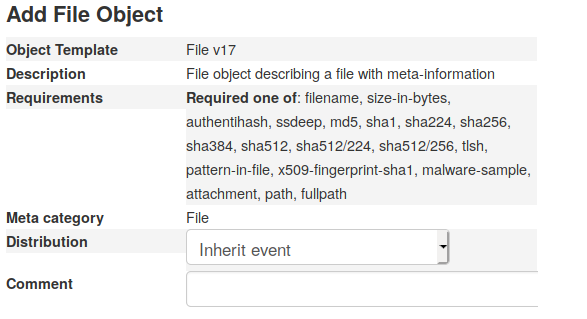
\includegraphics[scale=0.25]{fileobject.png}
\end{columns}
\end{frame}

